\graphicspath{{5series/asy/}}
\thispagestyle{empty}

\section{Series and the Theorems of Taylor \& Laurent}

The theory of series in complex analysis differs significantly from the real situation, particularly with regard to two concepts.
\begin{itemize}
  \item Taylor's Theorem:\quad Holomorphic functions \emph{equal} their Taylor series. This is false in real analysis where differentiable functions need not have, nor equal, a Taylor series.
  \item Laurent Series: series can also include negative powers such as $z^{-1}+3z^{-2}+\cdots$
\end{itemize}

Before discussing these concepts, we review the basic ideas of both infinite and power series: as we saw for sequences in Section \ref{sec:opensets}, this is essentially identical to the real situation.


\subsection{A Brief Review of Power Series}\label{sec:powerreview}


% 
% Post real analysis, there is little specific to say regarding sequences of complex numbers. The notions of limit, convergence and sequential continuity are essentially identical in $\C$ and $\R^2$. For instance:
% 
% \begin{defn}{}{}
% 	A sequence $(z_n)$ has limit $z\in\C$, written $\lim z_n=z$, if
% 	\[
% 		\forall\epsilon>0,\ \exists N\text{ such that }n>N\implies \nm{z_n-z}<\epsilon
% 	\]
% \end{defn}
% 
% Writing $z_n=x_n+ iy_n$ and $z=x+iy$ in real and imaginary parts, we see that
% \[
% 	\nm{z_n-z}\le\nm{x_n-x}+\nm{y_n-y}\le 2\nm{z_n-z}
% \]
% from which:
% 
% \begin{lemm}{}{limitcr}
% If $z_n=x_n+iy_n$, then $(z_n)$ converges if and only if both $(x_n)$ and $(y_n)$ converge, in which case
% \[\lim z_n=\lim x_n+i\lim y_n\]
% \end{lemm}
% 
% \textcolor{red}{Warning!}\quad While this mostly translates to the polar representation $z_n=r_ne^{i\theta_n}$, there is a caveat: the discontinuity of $\Arg z = \Theta$ when $z$ is a non-positive real number means that $(\Theta_n)$ need not converge even if $(z_n)$ does.
% 
% \begin{example}{}{}
% The sequence with $z_n=2i-\frac{1+i}n$ has limit $z=2i$: given $\epsilon>0$, let $N=\sqrt 2\epsilon$, then
% \[n>N\implies \nm{z_n-z}=\frac{\sqrt 2}n<\frac{\sqrt 2}N=\epsilon\]
% The real and imaginary parts are $x_n=-\frac 1n$ and $y_n=2-\frac 1n$ which clearly converge to $x=0$ and $y=2$ respectively. In polar co-ordinates things are also as expected
% \begin{gather*}
% \lim r_n=\lim\sqrt{\frac{1+(2n-1)^2}{n^2}}=\lim\frac 2n\sqrt{n^2-n}=2\\
% \lim\Theta_n=\lim\left(\pi\tan^{-1}\frac{(2n-1)/n}{-1/n}\right) =\pi+\tan^{-1}(1-2n)=\frac\pi 2
% \end{gather*}
% Since $z_n$ lies in the second quadrant and $z=2i$, we never get near the non-negative real axis where $\Theta_n$ is discontinuous.
% \end{example}

\begin{defn}{Infinite Series}{}
	The \emph{$n\th$ partial sum} of a sequence $(z_n)_{n=0}^\infty$ is the complex number
	\[
		s_n=\sum_{k=0}^nz_k=z_0+\cdots +z_n
	\]
	\vspace{-2pt}The \emph{(infinite) series} $\sum z_n:= \lim s_n$ is said to converge/diverge if the sequence $(s_n)$ converges/diverges.\smallbreak
	%If $\sum z_n$ is convergent, then the sequence of \emph{remainders} is defined by $\rho_n= \sum z_n- s_n$.\smallbreak
	The series \emph{converges absolutely} if $\sum \nm{z_n}$ converges.\smallbreak
	The series \emph{converges conditionally} if it converges but not absolutely.
\end{defn}

By convention, the initial term of the sequence/series is $z_0$. This isn't required: it could be $z_1$, etc.

\begin{thm}{Basic Series Facts}{seriesrc}
	Let $\sum z_n$ and $\sum w_n$ be series of complex numbers.
	\begin{enumerate}\itemsep0pt
	  \item If $z_n=x_n+iy_n$, then $\sum z_n$ converges if and only if $\sum x_n$ and $\sum y_n$ both converge, in which case
	  \[
	  	\sum z_n=\sum x_n+i\sum y_n
	  \]
	  \item\vspace{-3pt} If $a,b\in\C$, and $\sum z_n$ and $\sum w_n$ converge, then $\sum az_n+bw_n$ converges, in which case
	  \[
	  	\sum az_n+bw_n=a\sum z_n+b\sum w_n
	  \]
	  \item\vspace{-3pt} ($n\th$ term/divergence test)\lstsp If $\sum z_n$ converges, then $\lim z_n=0$.
	  \item The (real!) comparison, ratio and root tests apply to the series $\sum\nm{z_n}$.
	  \item Absolute convergence implies convergence; moreover $\nm{\sum z_n}\le\sum\nm{z_n}$.
	\end{enumerate}
\end{thm}

\begin{proof}
	\begin{enumerate}\itemsep0pt
	  \item This is Theorem \ref{thm:compbolzano}, part 1.
	  \item[2,]\negthickspace 3. \ These follow from 1 and the corresponding results for the real series $\sum x_n,\sum y_n$.
	  \setcounter{enumi}{3}
	  \item This requires no proof: $\sum \nm{z_n}$ is a series of non-negative real numbers, so the real version apply!
	  \item Since $\nm{x_n},\nm{y_n}\le\nm{z_n}$, the (real) comparison test says that $\sum x_n$ and $\sum y_n$ are absolutely convergent and thus convergent. By part 1, $\sum z_n$ converges. Finally, apply the triangle inequality $\nm{\sum\limits_{k=0}^m z_k}\le\sum\limits_{k=0}^m\nm{z_k}\le\sum\limits_{n=0}^\infty\nm{z_n}$ and take limits as $m\to\infty$.\qedhere
	\end{enumerate}
\end{proof}

\goodbreak
% 
% \begin{exercises*}
% \hangindent\leftmargini
% \textup{1.} \ Use the $\epsilon$-$N$ definition to prove that $\lim\frac{2+in}n= i$.
% \begin{enumerate}\setcounter{enumi}{1}
%   \item Give a rigorous proof of \ref{lemm:limitcr}. Sketch a proof of the corresponding statement for the polar representation whenever $\lim z_n$ is non-zero and not a negative real number.
%   
%   \item Explicitly prove part 2 of Theorem \ref{thm:seriesrc}.
%   
%   \item Fix $\theta\in (-\pi,\pi]$. Prove that the sequence defined by $z_n =e^{in\theta}$ converges if and only if $\theta = 0$.
%   
%   \item Use the $\epsilon$-$N$ definition to prove that $\lim\sqrt{i+\frac 1n}=\frac{1+i}{\sqrt 2}=\sqrt i$ where we use the principal value.%\par
%   %(\emph{Hint: The usual trick $\sqrt a-\sqrt b=\frac{a-b}{\sqrt a+\sqrt b}$ works, but be careful with complex conjugates!})
% \end{enumerate}
% \end{exercises*}
 

\begin{defn}{Power Series \& Analyticity}{}
	A \emph{power series centered at $z_0$} is a function of the form
	\[
		p(z)=\sum_{n=0}^\infty a_n(z-z_0)^n \tag{$z_0$ and the \emph{coefficients} $a_n$ are constants}
	\]
	A function $f:D\to\C$ is \emph{analytic} if every $z_0\in D$ has a neighborhood on which $f(z)$ equals a power series centered at $z_0$. That is,
	\[
		\forall z_0\in D,\ \exists\delta>0,\ (a_n)\text{ such that }\nm{z-z_0}<\delta\implies f(z)=\smash[t]{\sum_{n=0}^\infty} a_n(z-z_0)^n
	\]
	To be analytic at a point $z_0$ is to be analytic on some neighborhood of $z_0$.
\end{defn}


\begin{example}{Geometric series}{geomseries}
	By the $n\th$ term test, the power series $\sum\limits z^n$ diverges when $\nm z\ge 1$. Otherwise, inside the unit circle $\nm z<1$ we have $z^{n+1}\to 0$, from which
	\[
		s_n-zs_n=1-z^{n+1}\implies s_n=\frac{1-z^{n+1}}{1-z} \implies \sum\limits_{n=0}^\infty z^n =\lim s_n=\frac 1{1-z}
	\]
	In fact $f(z)=\frac 1{1-z}$ is analytic on its whole domain $\C\setminus\{1\}$: the substitution $z\mapsto\frac{z-z_0}{1-z_0}$ ($z_0\neq 1$) to see that $\frac 1{1-z}$ equals a power series centered at $z_0$:
	\[
		\frac 1{1-z} =\frac 1{1-z_0}\cdot \frac 1{1-\frac{z-z_0}{1-z_0}}=\frac 1{1-z_0}\sum_{n=0}^\infty \left(\frac{z-z_0}{1-z_0}\right)^n
		\quad\text{whenever}\quad
		\nm{z-z_0}<\nm{1-z_0}
	\]
\end{example}

Regardless of the center $z_0$, observe how the geometric series converges on a \emph{disk} (radius $\nm{1-z_0}$). This behavior in fact happens for \emph{every} power series, analogous to the interval/radius of convergence discussion from real analysis.


\begin{thm}[lower separated=false, sidebyside, sidebyside align=top seam, sidebyside gap=0pt, righthand width=0.23\linewidth]{Radius of Convergence}{absconv}
	Suppose $p(z)=\sum a_n(z-z_0)^n$.
	\begin{enumerate}
	  \item If $p(z)$ converges at $z_1\neq z_0$, then it is absolutely convergent at every \textcolor{red}{every $z$} satisfying $\nm{z-z_0}<\nm{z_1-z_0}$.
		\item Define the \textbf{radius of convergence} $R_0:=\sup\bigl\{\nm{z-z_0}: p(z) \text{ converges}\bigr\}$. Then $p(z)$ converges absolutely whenever $\nm{z-z_0}<R_0$, and diverges whenever $\nm{z-z_0}>R_0$.
	\end{enumerate}
	\tcblower
	\flushright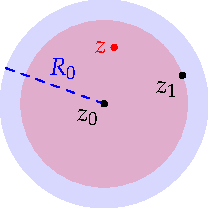
\includegraphics[scale=0.95]{conv}
\end{thm}



\begin{proof}
	\begin{enumerate}
	  \item By the $n\th$ term test, the sequence $\bigl(a_n(z_1-z_0)^n\bigr)$ converges (to 0); it is therefore bounded by some $M\in\R^+$. But then
		\[
			\nm{a_n}\nm{z-z_0}^n
			=\nm{a_n}\nm{z_1-z_0}^n\left(\frac{\nm{z-z_0}}{\nm{z_1-z_0}}\right)^n
			\le Mr^n
			\quad\text{where}\quad 
			r=\frac{\nm{z-z_0}}{\nm{z_1-z_0}}<1
		\]
		Since $\sum Mr^n$ converges, the comparison test says that $\sum\nm{a_n}\nm{z-z_0}^n$ converges.
		\item If $\nm{z-z_0}<R_0$, then $\exists z_1$ such that $\nm{z-z_0}<\nm{z_1-z_0}\le R_0$ and $p(z_1)$ converges; now apply part (a). The divergence condition is an exercise.\qedhere
	\end{enumerate}
\end{proof}

A power series therefore has a \emph{disk of convergence.} As in real analysis, we have to test convergence separately on the boundary circle $\nm{z-z_0}=R_0$; a key technique for this is \emph{Abel's Test} (Exercise \ref{exs:abeltest}). Note particularly the two extreme cases:
\begin{itemize}%\itemsep2pt
	\item If $R_0=\infty$, the series is absolutely convergent on $\C$.
	\item If $R_0=0$, the series converges only when $z=z_0$.
\end{itemize}
As in real analysis, we could also compute $R_0=\liminf\nm{a_n}^{-1/n}$, though for us this will mostly be redundant since the condition observed in Exercise 1 (proved generally in Section \ref{sec:unifconv}) is often obvious. %We will typically try to compute a power series representation for a given function $f(z)$ and, as we'll later observe, $R_0$ is simply the distance from $z_0$ to the nearest point at which $f$ fails to be differentiable.

\begin{exercises}
	\exstart Sketch the disks of convergence with centers $z_0=-1$, $1+i$, $3-2i$ for the function $f(z)=\frac 1{1-z}$ (Example \ref{ex:geomseries}). Complete the following observation:\vspace{-5pt}
	
	\begin{enumerate}\setcounter{enumi}{1}
		\item[]\begin{quote}
			$R_0=\nm{1-z_0}$ is the distance from $z_0$ to the nearest point at which $f(z)$ is \underline{\phantom{undefineddd}}
		\end{quote}
		
	  \item By mimicking Example \ref{ex:geomseries}, find a power series centered at $z_0\neq i$ which equals the function $g(z)=\frac 2{1+iz}$. What is its radius of convergence?
	  
  	\item Revisit the proof of Theorem \ref{thm:absconv}.
  	\begin{enumerate}
  	  \item Complete part 2: If $\nm{z-z_0}>R_0$, prove that $p(z)=\sum a_n(z-z_0)^n$ diverges.
  	  \item In part 1, explain why we couldn't simply use the comparison test to say
	  	\[
	  		\nm{a_n}\nm{z-z_0}^n<\nm{a_n}\nm{z_1-z_0}^n\implies \sum\nm{a_n}\nm{z-z_0}^n\text{ converges}
	  	\]
	  	(\emph{Hint: Think carefully about the hypothesis!})
	  \end{enumerate}
	  
	  \item\label{exs:abeltest} (\emph{Abel's Test})\lstsp In real analysis, the alternating series test was often used to decide convergence at the endpoints of an interval of convergence. Here is a generalization to the complex situation.\par
	  Consider the power series $\sum a_nz^n$ where $(a_n)$ is a \emph{real} sequence such that
	  \[
	  	a_n\ge 0,\quad a_{n+1}\le a_n,\quad \lim_{n\to\infty}a_n=0
	  \]
	  \begin{enumerate}
	    \item Write $\smash{s_n(z)=\sum\limits_{k=0}^na_kz^k}$ for the partial sum and prove that
	    \[
	    	(1-z)s_n(z)=a_0-a_nz^{n+1}+\sum_{k=1}^n(a_k-a_{k-1})z^k
	    \]
	    
	    \item Prove \emph{Abel's Test}: $\sum a_nz^n$ converges on the \emph{closed} disk $\nm z\le 1$, \emph{except perhaps} when $z=1$.\par
	    (\emph{Hint: Show that $\sum(a_k-a_{k-1})z^k$ converges absolutely by comparison with a telescoping series})
	    
	    \item\begin{enumerate}
	      \item Find the disk of convergence of $\sum\frac{z^n}n$ (all $z\in\C$ at which the series converges).
	    	\item Prove that the real series $\sum\frac{\cos n\theta}n$ converges except when $\theta$ is divisible by $2\pi$. For what values of $\theta$ does the series $\sum\frac{\sin n\theta}n$ converge?\par
	    	(\emph{Hint: Use part (i)\ldots})
	   	\end{enumerate}
	    
	    \item Find all values of $z$ for which the series $\sum \frac{1+i}{(n+i)(4+3i)^n}(z-1+2i)^n$ converges and sketch the disk of convergence.\par
	    (\emph{Hint: Let $w=\frac{z-1+2i}{4+3i}$ and think about real and imaginary parts})
	  \end{enumerate}
	\end{enumerate}
	
\end{exercises}


\clearpage



\subsection{Taylor Series and Taylor's Theorem}

The overarching goal of the next two sections is the establishment of a key result:
\[
	\tcbhighmath{\text{A function is holomorphic if and only if it is analytic}}
\]
Otherwise said, $f(z)$ is differentiable on an open domain $D$ if and only if for each $z_0\in D$ there is some neighborhood of $z_0$ on which it equals a power series $f(z)=\sum a_n(z-z_0)^n$.\smallbreak

If a holomorphic function is to equal a power series, it is natural ask \emph{which one}? The answer revisits a familiar definition and leads to a startling difference between the real and complex cases.

\begin{defn}{}{}
	If $f(z)$ is infinitely differentiable at $z_0$, then its \emph{Taylor series} is the power series
	\[
		\sum_{n=0}^\infty a_n(z-z_0)^n= \sum_{n=0}^\infty \frac{f^{(n)}(z_0)}{n!}(z-z_0)^n
	\]
	The \emph{Taylor coefficients} are $a_n=\frac{f^{(n)}(z_0)}{n!}$. A \emph{Maclaurin series} is a Taylor series centered at $z_0=0$.
\end{defn}

\begin{example*}[exstyle,lower separated=false, sidebyside, sidebyside align=top seam, sidebyside gap=0pt, righthand width=0.26\linewidth]{\ref{ex:geomseries}, cont.}{}
	On the disk $\nm z<1$, the function $f(z)=\frac 1{1-z}$ has 
  \[
  	f^{(n)}(z)=\frac{n!}{(1-z)^{n+1}}\implies \sum\limits_{n=0}^\infty\frac{f^{(n)}(0)}{n!}z^n =\sum\limits_{n=0}^\infty z^n = f(z)
  \]
  The Maclaurin series is precisely the geometric power series representation of $f(z)$ on the open disk $\nm z<1$!\smallbreak
  In complex analysis, this situation is completely general\ldots
	\tcblower
  \flushright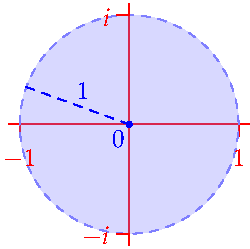
\includegraphics[scale=0.9]{taylorex1}
\end{example*}


\begin{thm}{Taylor's Theorem}{taylor}
	Suppose $f(z)$ is holomorphic on a disk $\nm{z-z_0}<R$. Then,
	\[
		f(z)=\sum_{n=0}^\infty \frac{f^{(n)}(z_0)}{n!}(z-z_0)^n
		\quad\text{whenever}\quad
		\nm{z-z_0}<R
	\]
\end{thm}

In comparison to real analysis, this is a \emph{very} strong statement: in the real case, Taylor's Theorem is usually stated with one of several awkward remainder terms, and there exist infinitely differentiable functions which do not equal their Taylor series (see Exercise \ref{ex:maczero}).\smallbreak
Plainly $R$ cannot be larger than the radius of convergence $R_0$ of the Taylor series. If $f$ is entire, then the result holds for all positive $R$ and the series has infinite radius of convergence.

\begin{examples}{}{}
	Familiar Maclaurin series are identical to real analysis:
	\[
		e^z=\sum\limits_{n=0}^\infty\frac{z^n}{n!}\qquad
		\sin z=\sum\limits_{n=0}^\infty\frac{(-1)^n}{(2n+1)!}z^{2n+1}\qquad
		\cos z=\sum\limits_{n=0}^\infty\frac{(-1)^n}{(2n)!}z^{2n}
	\]
	Since $e^z$, $\sin z$ and $\cos z$ are entire, we may take $R=\infty$ in Taylor's Theorem: each function equals its Maclaurin series everywhere on $\C$.
\end{examples}

\goodbreak

Before seeing the proof of Taylor's Theorem, we apply it to quickly deduce half of our key result.\smallbreak
If $f:D\to\C$ is holomorphic, then, for every $z_0\in D$, there exists some disk $\nm{z-z_0}<R$ on which $f$ is holomorphic. By Taylor's Theorem, $f(z)$ equals its Taylor series on this disk. Otherwise said:

\begin{cor}{}{}
	Every holomorphic function is analytic.
\end{cor}

We'll obtain the converse in the next section.\bigbreak

Why is Taylor's Theorem so much more specific in complex analysis? The reason is that we have can apply a powerful tool unavailable in real analysis: Cauchy's integral formula.

\begin{proof}[Proof of Taylor's Theorem]
	By relabelling $\tilde f(z)=f(z-z_0)$, it is enough to prove when $z_0=0$, that is for Maclaurin series. We therefore suppose $f(z)$ is holomorphic when $\nm z<R$.\par
	\begin{minipage}[t]{0.7\linewidth}\vspace{-2pt}
		Let $w$ be given where $\nm w<R$. Apply the geometric series formula (Example \ref{ex:geomseries}), to see that if $z\neq 0$, then
		\[
			\frac 1z\sum_{k=0}^{n-1}\left(\frac wz\right)^k
			=\frac{1-\left(\frac wz\right)^n}{z(1-\frac wz)} 
			=\frac 1{z-w}-\frac 1{z-w}\left(\frac wz\right)^n
			\tag{$\ast$}
		\]
		Choose any circle $C_r$ centered at the origin whose radius satisfies $\nm w<r<R$. Since both $0$ and $w$ lie inside $C_r$, we may apply Cauchy's integral formula \emph{twice}:
	\end{minipage}
	\hfill
	\begin{minipage}[t]{0.29\linewidth}\vspace{-2pt}
		\flushright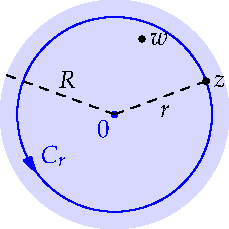
\includegraphics[scale=0.95]{taylor}
	\end{minipage}\par
	\vspace{-6pt}
	\begin{align*}
		f(w)
		&=\frac 1{2\pi i}\oint_{C_r}\frac{f(z)}{z-w}\dz
			\tag{Cauchy for $C_r$ around $w$}\\
		&=\sum_{k=0}^{n-1}\frac{w^k}{2\pi i}\oint_{C_r}\frac{f(z)}{z^{k+1}}\,\dz
			+\frac{w^n}{2\pi i}\oint_{C_r}\frac{f(z)}{z^n(z-w)}\,\dz
			\tag{subsititute for $\frac 1{z-w}$ using $(\ast)$}\\
	 	&=\sum_{k=0}^{n-1} \frac{f^{(k)}(0)}{k!}w^k 
	 		+\frac{w^n}{2\pi i}\oint_{C_r}\frac{f(z)}{z^n(z-w)}\,\dz
	 		\tag{Cauchy for $C_r$ around $0$}
	\end{align*}
	To finish the proof, we must control the final integral. Since $f$ is holomorphic on $C_r$, it is bounded by some $M>0$. Moreover, for $z\in C_r$ we have $\nm{z-w}\ge \nm{\nm z-\nm w}= r-\nm w$. It follows that
	\begin{align*}
		\nm{f(w)-\sum_{k=0}^{n-1} \frac{f^{(k)}(0)}{k!}w^k}
			&=\frac{\nm w^n}{2\pi}\nm{\oint_{C_r}\frac{f(z)}{z^n(z-w)}\,\dz}\\
			&\le\frac{\nm w^nM\cdot 2\pi r}{2\pi r^n(r-\nm w)}
				=\frac{Mr}{(r-\nm w)}\left(\frac{\nm w}r\right)^n 
	\end{align*}
	Since $\nm w<r$, this last converges to zero. Otherwise said
	\[
		f(w)=\lim_{n\to\infty}\sum_{k=0}^{n-1} \frac{f^{(k)}(0)}{k!}w^k 
		=\sum_{n=0}^{\infty} \frac{f^{(n)}(0)}{n!}w^n
	\]
	so that $f(w)$ equals its Maclaurin series whenever $\nm w<R$.
\end{proof}


\begin{example}{}{logtaylori}
	The principal logarithm $f(z)=\Log z$ is holomorphic on the open disk $\nm{z-i}<1$.\par
  \begin{minipage}[t]{0.7\linewidth}\vspace{0pt}
  	Whenever $n\ge 1$, we have
		\[
			f^{(n)}(i)
			=\at{\frac{(-1)^{n-1}(n-1)!}{z^{n}}}{z=i}
			=-i^n(n-1)!
		\]
		By Taylor's Theorem, $f(z)$ equals its Taylor series on the disk:
  	\[
  		\Log z=\Log i-\sum_{n=1}^\infty \frac{i^n}{n}(z-i)^n =\frac{\pi i}2-\sum_{n=1}^\infty \frac{(iz+1)^n}n
  	\]
  \end{minipage}
  \hfill
  \begin{minipage}[t]{0.29\linewidth}\vspace{0pt}
  	\flushright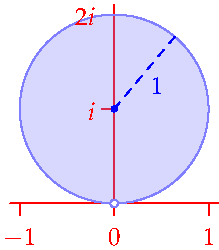
\includegraphics{taylorex2}
  \end{minipage}\medbreak
  
	In case you're feeling skeptical, convergence \emph{inside} the disk ($\nm{z-i}<1$) can be verified directly using the comparison test:
	\[
		\nm{z-i}=r<1\implies\frac{\nm{z-i}^n}n\le r^n\implies \sum\frac{i^n(z-i)^n}n\text{ converges absolutely}
	\]
	At $z=0$, we recognize the divergent harmonic series $\sum \frac 1n$, so the radius of convergence of the Taylor series is in fact $R_0=1$. Exercise \ref{exs:abel2} shows that the series converges everywhere else on the boundary circle $\nm{z-i}=1$.
\end{example}


\begin{exercises}
	\hangindent\doubleind
	\textup{1.} \ (a) \ Compute the Maclaurin series of $\cos z$ directly from the definition.
	\begin{enumerate}\setcounter{enumi}{1}
	  \item[]\begin{enumerate}\setcounter{enumii}{1}\vspace{-3pt}
	    \item Evaluate the Taylor series of $\sin z$ about $z_0=\frac\pi 2$ and confirm that it equals your answer to part (a) when $z$ is replaced with $z-\frac\pi 2$.
	    
	    \item Find the Taylor series of $\cos z$ centered at $z_0=i$.
	  \end{enumerate} 
	  
	  
	  \item Consider $f(z)=\frac 1z$. For any $z_0\neq 0$, find the Taylor series of $f(z)$ about $z_0$. What is its disk of convergence?
	  	  
	  
	  \item\label{exs:abel2} Use Abel's test (Exercise \ref*{sec:powerreview}.\ref{exs:abeltest}) to verify that the Taylor series for $\Log z$ centered at $z_0=i$ (Example \ref{ex:logtaylori}) converges everywhere on the boundary circle $\nm{z-i}=1$, except when $z=0$.

	    
	  \item\label{ex:maczero} Consider the function
	  \[
	  	f(z)=
	  	\begin{cases}
	  		e^{-1/z^2}&\text{if }z\neq 0\\
	  		0&\text{if }z=0
	  	\end{cases}
	  \]
	  When $z\in\R$ this provides the classic example of an infinitely differentiable function whose Maclaurin series (being identically zero) does not equal the original function except at the origin. When $z\in\C$, explain why $f(z)$ does not contradict Taylor's Theorem.
	  
	\end{enumerate}
\end{exercises}
\clearpage



\subsection{Uniform Convergence: Continuity, Integrability and Differentiability}\label{sec:unifconv}

As in real analysis, we'd like to establish three useful facts:
\begin{enumerate}
  \item Representations are unique: if two power series are equal, their coefficients are equal.
  \item Power series are continuous, indeed differentiable, inside their disk of convergence.
  \item Power series may be differentiated and integrated term-by-term.
\end{enumerate}

The arguments are intertwined. Since these are often similar or identical to the real case, we will be brief and postpone all examples until the end. The critical ingredient is uniform convergence.

\begin{defn}{}{}
	Suppose $f(z)=\sum a_n(z-z_0)^n$ is a power series with $n\th$ partial sum $s_n(z)$ and remainder $\rho_n(z) = f(z) - s_n(z)$. We say that the series \emph{converges uniformly} on a domain $D$ if
	\[
		\forall\epsilon>0,\ \exists N\text{ such that }n>N,\ z\in D\implies \nm{\rho_n(z)}<\epsilon
	\]
\end{defn}

\emph{Uniformity} means that $N=N(\epsilon)$ is independent of the location $z\in D$. If $N=N(\epsilon,z)$ were permitted to depend on $z$, we'd refer to the convergence as \emph{pointwise.}

\begin{thm}{}{unifconv}
	Let $R_0$ be the radius of convergence of a power series centered at $z_0$. If $R_1<R_0$, then the series converges uniformly on the closed disk $\nm{z-z_0}\le R_1$.
\end{thm}

This first argument also applies in real analysis.

\begin{proof}
	As preparation, suppose $z_1$ satisfies $\nm{z_1-z_0}=R_1$. Since $R_1<R_0$, the series converges absolutely at $z_1$ (Theorem \ref{thm:absconv}). Denote by $\sigma_n$ the $n\th$ remainder of this absolutely convergent series:\par
	\begin{minipage}[t]{0.7\linewidth}\vspace{-8pt}
	\[
		\sigma_n=\sum_{k=n+1}^\infty\nm{a_k}\nm{z_1-z_0}^k =\sum_{k=n+1}^\infty\nm{a_k}R_1^k
	\]
	Now suppose $\epsilon>0$ is given. Since the above series converges, the $n\th$-term test says that $\lim\limits_{n\to\infty}\sigma_n=0$: that is,
	\[
		\exists N\text{ such that }n>N\implies \sigma_n<\epsilon
	\]
	By the comparison test, if $z$ satisfies $\nm{z-z_0}\le R_1$, then
	\end{minipage}
	\hfill
	\begin{minipage}[t]{0.29\linewidth}\vspace{0pt}
		\flushright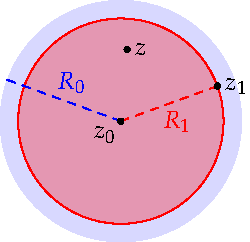
\includegraphics[scale=0.95]{uniform}
	\end{minipage}\par\vspace{-4pt}
	\[
		\nm{\rho_n(z)} =\nm{\sum_{k=n+1}^\infty a_k(z-z_0)^k}
		\le\sum_{k=n+1}^\infty\nm{a_k}\nm{z-z_0}^k 
		\le\sum_{k=n+1}^\infty\nm{a_k}R_1^k
		=\sigma_n <\epsilon
	\]
	Since $N$ depends only on $\epsilon$ (not on $z$), we conclude that the convergence is uniform.\footnotemark
\end{proof}

\footnotetext{%
	It looks as if $N$ might also depend on the choice of $z_1$ in the first line. However, any suitable $z_1$ produces the same value $R_1=\nm{z_1-z_0}$ and thus the same sequence $(\sigma_n)$. It is from the convergence of this sequence that we get $N$.%
}

That $R_1$ is \emph{strictly less} than the radius of convergence $R_0$ is important. In Exercise \ref{ex:notuniform}, we'll see that a power series need not converge uniformly on the full open disk of convergence $\nm{z-z_0}<R_0$.

\goodbreak

\begin{thm}{Continuity}{seriescont}
	Suppose $f(z)=\sum a_n(z-z_0)^n$ has radius of convergence $R_0$. Then $f(z)$ is continuous on the open disk of convergence $\nm{z-z_0}<R_0$.
\end{thm}

This is identical to the famous $\frac\epsilon 3$-proof encountered in real analysis.

\begin{proof}
	Fix $w$ and $R_1$ such that $\nm{w-z_0}<R_1<R_0$. Let $\epsilon>0$ be given. Observe:\par
	\begin{minipage}[t]{0.7\linewidth}\vspace{0pt}
		\begin{itemize}\itemsep0pt
			\item Uniform convergence whenever $\nm{z-z_0}\le R_1$ (Theorem \ref{thm:unifconv}):
			\[
				\exists N\text{ such that }n>N\implies \nm{\rho_n(z)}<\frac\epsilon 3\text{ and }\nm{\rho_n(w)}<\frac\epsilon 3
			\]
		  \item Openness and continuity ($s_n$ is a polynomial!): for any $n>N$,
		  \[
		  	\exists\delta>0\text{ such that } \nm{z-w}<\delta\implies
		  	\begin{cases}
		  		\nm{z-z_0}<R_1\\
					\nm{s_n(z)-s_n(w)}<\frac\epsilon 3
		  	\end{cases}
		  \]
		\end{itemize}
	\end{minipage}
	\hfill
	\begin{minipage}[t]{0.29\linewidth}\vspace{-6pt}
		\flushright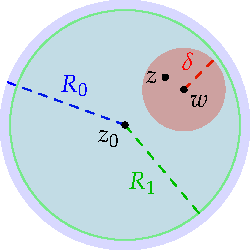
\includegraphics[scale=0.95]{cont}
	\end{minipage}\medbreak
	Put everything together to see that $f(z)$ is continuous at $w$: for any $n>N$,
	\begin{align*}
		\nm{z-w}<\delta\implies \nm{f(z)-f(w)}
			&=\nm{f(z)-s_n(z)+s_n(z)-s_n(w)+s_n(w)-f(w)}\\
			&\le \nm{\rho_n(z)}+\nm{s_n(z)-s_n(w)}+\nm{\rho_n(w)}
			<\epsilon
			\tag*{\qedhere}
	\end{align*}
\end{proof}

The discussion now differs from the real approach via our employ of \emph{contour integrals.} The remaining results follow from a general version of term-by-term integration.

\begin{thm}[lower separated=false, sidebyside, sidebyside align=top seam, sidebyside gap=0pt, righthand width=0.25\linewidth]{}{inttermbyterm}
	Suppose $f(z)=\sum a_n(z-z_0)^n$ has radius of convergence $R_0$. Let $g(z)$ be continuous on some contour $C$ in the open disk of convergence $\nm{z-z_0}<R_0$. We may then integrate term-by-term:
	\[
		\int_Cg(z)f(z)\,\dz=\sum_{n=0}^\infty a_n\int_C g(z)(z-z_0)^n\,\dz
	\]
	\tcblower
	\flushright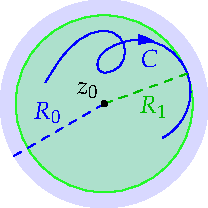
\includegraphics[scale=0.95]{cont2}
\end{thm}

\begin{proof}
	The integral $\int_C g(z)f(z)\,\dz$ exists since $f,g$ are continuous on $C$. Since $C$ is a compact set:
	\begin{itemize}
	  \item $C$ lies in some closed disk $\nm{z-z_0}\le R_1<R_0$ on which the series $f(z)$ converges uniformly.
	  \item $g(z)$ is bounded on $C$ by some $M>0$.
	\end{itemize}
	Let $C$ have length $L$ and let $\epsilon>0$ be given. Since $f(z)$ converges uniformly when $\nm{z-z_0}\le R_1$,
	\[
		\exists N\text{ such that }n>N\implies \nm{\rho_n(z)}<\frac\epsilon{ML}
	\]
	Now take integrals and moduli; if $n>N$, then
	\begin{align*}
		\nm{\int_Cg(z)f(z)\,\dz-\sum_{k=0}^n a_k\int_C g(z)(z-z_0)^k\,\dz}
		&=\nm{\int_C g(z)\left(f(z)-\sum_{k=0}^n a_k(z-z_0)^k\right)\,\dz}\\
		&=\nm{\int_C g(z)\rho_n(z)\,\dz}
		< M\cdot\frac{\epsilon}{ML}\cdot L=\epsilon \tag*{\qedhere}
	\end{align*}
\end{proof}


\goodbreak


Everything we want now follows by choosing specific functions $g(z)$ in Theorem \ref{thm:inttermbyterm}!

\begin{cor}{}{contintdiff}
	Suppose $f(z)=\sum a_n(z-z_0)^n$ has positive radius of convergence $R_0$.
	\begin{enumerate}\itemsep0pt
	  \item (Term-by-term integration)\quad Let $g(z)=1$ to see that
	  \[
	  	\int_Cf(z)\,\dz=\sum_{n=0}^\infty a_n\int_C (z-z_0)^n\,\dz =\sum_{n=0}^\infty\frac{a_n}{n+1}(z-z_0)^{n+1}\bigg|_{C(\text{start})}^{C(\text{end})}
	  \]
	  
	  \item (Holomorphicity)\quad By part 1, $\int_Cf$ is path-independent for any contour $C$ in the open disk of convergence. We conclude (Summary, page \pageref{pg:ftcsummary}) that $f$ is holomorphic on said disk. In particular, \textbf{every analytic function is holomorphic}.
	  
		\begin{minipage}[t]{0.78\linewidth}\vspace{0pt}
		  \item (Term-by-term differentiation)\quad Given $\nm{w-z_0}<R_0$, let $g(z)=\frac 1{2\pi i(z-w)^2}$ and apply Cauchy's integral formula on a \textcolor{red}{small circle} around $w$:
		  \begin{align*}
		  	f'(w)&=\frac 1{2\pi i}\oint_C\frac{f(z)}{(z-w)^2}\,\dz 
		  		=\sum \frac{a_n}{2\pi i}\oint_C\frac{(z-z_0)^n}{(z-w)^2}\,\dz\\
		  	&=\sum a_n\diffat{z}{z=w}(z-z_0)^n 
		  		=\sum a_nn(w-z_0)^{n-1}
		  \end{align*}
		\end{minipage}
		\hfill
		\begin{minipage}[t]{0.21\linewidth}\vspace{-5pt}
			\flushright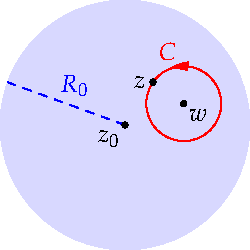
\includegraphics[scale=0.95]{diff}
		\end{minipage}
		
		\item\label{thm:contintdiff4} (Unique representation)\quad The power series is the Taylor series of $f(z)$: that is, $a_n=\frac{f^{(n)}(z_0)}{n!}$.
	\end{enumerate}
\end{cor}

In Exercise \ref{ex:uniquetaylor} proves unique representation. Since analytic and holomorphic are now equivalent, we'll retire the latter term for the rest of these notes. 

\begin{examples}{}{}
	We may now compute Taylor \& Maclaurin series using algebra, integration and differentiation: if a function equals a series, that's the one we want regardless of how we found it!
	\begin{enumerate}
	  \item $f(z)=z^3e^{z^2}=z^3$ \scalebox{0.9}{$\displaystyle\sum\limits_{n=0}^\infty\frac{(z^2)^n}{n!}$}\,$\mathrel{=}$\,\scalebox{0.9}{$\displaystyle\sum\limits_{n=0}^\infty\frac{z^{2n+3}}{n!}$} is the Maclaurin series of $f(z)$. Since the radius of convergence is infinite, the function equals its Maclaurin series everywhere on $\C$.
	  
	  \item The function $f(z)=
	  \begin{cases}
	  	\frac{\sin z}z&\text{if }z\neq 0\\
	  	1&\text{if }z=0
	  \end{cases}\ $
	  is entire since it equals the power series $\sum\limits_{n=0}^\infty\frac{(-1)^n}{(2n+1)!}z^{2n}$.
	  
	  \begin{minipage}[t]{0.7\linewidth}\vspace{0pt}
		  \item We find the Maclaurin series of $f(z)=\frac 1{z^4+16i}$ algebraically:
		  \[
		  	f(z)=\frac 1{16i\left(1-\frac{z^4}{-16i}\right)} 
		  	=\frac 1{16i}\sum_{n=0}^\infty\left(\frac{z^4}{-16i}\right)^n 
		  	=\sum_{n=0}^\infty\frac{i^{n-1}}{16^{n+1}}z^{4n}
		  \]
		  This converges whenever $\nm{\frac{z^4}{-16i}}<1\Longleftrightarrow \nm z<2$, equalling the distance from the center to the \textcolor{Green}{nearest point(s)} where $f(z)$ is undefined. If $C$ is the \textcolor{blue}{straight line} from $z=0$ to $z=1+i$, then
	  \end{minipage}
	  \hfill
	  \begin{minipage}[t]{0.29\linewidth}\vspace{0pt}
	  	\flushright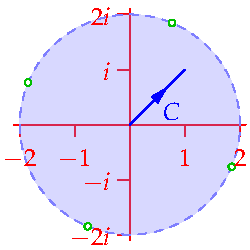
\includegraphics[scale=.95]{taylorex3}
	  \end{minipage}\par  
	  \[
	  	\int_Cf(z)\,\dz
	  	=\sum_{n=0}^\infty\frac{i^{n-1}}{16^{n+1}}\int_Cz^{4n}\,\dz 
	  	=\sum_{n=0}^\infty\frac{i^{n-1}(1+i)^{4n+1}}{16^{n+1}(4n+1)} 
	  	=\sum_{n=0}^\infty\frac{1-i}{16(4n+1)}\left(\frac{-i}{4}\right)^n
	  \] 
	\end{enumerate}
\end{examples}


\goodbreak


\begin{exercises}
	\exstart Find a power series representation and the radius of convergence:
	\begin{enumerate}\setcounter{enumi}{1}
	  \item[]\begin{enumerate}
	    \item $f(z)=\dfrac z{4-z}$ about $z_0=0$
	    \qquad\qquad
	    (b) \ $f(z)=z\sin z^2$ about $z_0=0$
	    \setcounter{enumii}{2}
	    \item $f(z)=\cosh 3z$ about $z_0=\dfrac{i\pi}9$
		\end{enumerate}
		
		
		\item\begin{enumerate}
		  \item \emph{Without computing derivatives}, find the Taylor series for $f(z)=\frac 1z$ about $z_0\neq 0$.
		  \item Differentiate your answer term-by-term to find the Taylor series of $\frac 1{z^2}$ about $z_0$.
		\end{enumerate} 
		
		
		\item By expressing $f(z)$ as a Maclaurin series, show that it is entire:
		\[
			f(z)=
			\begin{cases} 
				\frac 1{z^2}(1-\cos z)&\text{if }z\neq 0\\
				\frac 12&\text{if }z=0
			\end{cases}
		\]
		
		
		\item\begin{enumerate}
		  \item By integrating the Taylor series for $z^{-1}$ about $z_0=1$, prove that 
		  \[
		  	\Log z=\sum_{n=1}^\infty\frac{(-1)^{n+1}}n(z-1)^n
		  	\quad\text{whenever }\nm{z-1}<1
		  \]
		  \item Prove that the following function is analytic on the domain $0<\nm z$, \ $\Arg z\in(-\pi,\pi)$:
		  \[
		  	f(z)=
		  	\begin{cases} 
					\frac{\Log z}{z-1}&\text{if }z\neq 1\\
					1&\text{if }z=1
				\end{cases}
			\]
		\end{enumerate}
		
		
		\item Consider the Maclaurin series $f(z)=\sum_{n=0}^\infty (-1)^nz^{2n}$ on the disk $\nm z<1$. Show that $h(z)=\frac 1{z^2+1}$ is the analytic continuation (Definition \ref{defn:analyticcont}) of $f(z)$ to $\C\setminus\{i,-i\}$. 
		
		
		\item\label{ex:uniquetaylor}\begin{enumerate}
		  \item Prove part 4 of Corollary \ref{cor:contintdiff}: if $f(z)= \sum a_n(z-z_0)^n$, prove that $f^{(m)}(z_0)=m!a_m$ so that the series really is the Taylor series of $f(z)$.\par
			(\emph{Hint: let $g(z) =\frac{m!}{2\pi i(z-z_0)^{m+1}}$ in Theorem \ref{thm:inttermbyterm}})
			\item Explain carefully why every power series defines an analytic function.\par
	  (\emph{Think carefully about the definitions and what we've proved in the last two sections!})
		\end{enumerate}
		
		
		\item\label{exs:raddistnonanalytic} Suppose that the series $\sum a_n(z-z_0)^n$ has radius of convergence $R_0$ and that $f(z)=\sum a_n(z-z_0)^n$ whenever $\nm{z-z_0}<R_0$. Prove that
		\[
			R_0=\inf\bigl\{\nm{\hat z-z_0}:f(z)\text{ non-analytic or undefined at $\hat z$}\bigr\}
		\]
		(\emph{$R_0$ is essentially the distance from $z_0$ to the nearest point at which $f(z)$ is non-analytic})
		
		
		\item\label{ex:notuniform} (Hard)\lstsp Consider $f(z)=\frac 1{1-z}=\sum\limits_{n=0}^\infty z^n$ on $\nm z<1$.
		\begin{enumerate}
		  \item Let $R_1<1$. Explicitly check uniform convergence when $\nm z\le R_1$. That is, given $\epsilon>0$, find an explicit $N$ such that
		  \[
		  	n>N\implies \nm{\rho_n(z)}=\biggl|f(z)-\sum_{k=0}^nz^k\biggr|<\epsilon\text{ whenever }\nm z\le R_1
		  \]
		  \item Prove that $f(z)$ is \emph{not} uniformly convergent on $\nm z<1$.\par
		  (\emph{Hint: Let $\epsilon=1$ and aim for a contradiction\ldots})
		\end{enumerate}
	\end{enumerate}
\end{exercises}


\clearpage


\subsection{Laurent Series}

While Taylor series are undeniably useful, they also have weaknesses, not least because their domains are \emph{disks.} We motivate a more general construction with an example.

\begin{example}{}{laurentmotiv}
	$f(z)=\frac 1{z(2-z)}$ can be written as a Taylor series centered at $z=1$:\par
	\begin{minipage}[t]{0.7\linewidth}\vspace{-10pt}
		\[
			f(z)=\frac 1{1-(z-1)^2} 
			=\sum_{n=0}^\infty (z-1)^{2n}
			\quad\text{whenever \ \textcolor{Green}{$\nm{z-1}<1$}}
		\]
		However, we are also interested in the behavior of $f(z)$ near the points $z=0,2$. Due to their disk-domains, we can't use Taylor series to loop around these points.\smallbreak
		As an alternative, start with the Maclaurin series for $\frac 1{2-z}$ (valid when $\nm z<2$) and divide through by $z$ to obtain a new expression:
	\end{minipage}
	\hfill
	\begin{minipage}[t]{0.29\linewidth}\vspace{-10pt}
		\flushright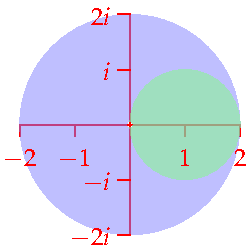
\includegraphics[scale=0.95]{laurent}
	\end{minipage}\par\vspace{-10pt}
	\begin{align*}
		f(z)&=\frac 1{2z(1-\frac{z}{2})}
		=\frac 1{2z}\sum_{n=0}^\infty\left(\frac z2\right)^n 
		=\sum_{n=-1}^\infty\frac{z^n}{2^{n+2}}\\
		&=\frac 1{2z}+\frac 14+\frac z8+\frac{z^2}{16}+\frac{z^3}{32}+\cdots	
	\end{align*}
	By construction, this `series with negative terms' is valid on the \textcolor{blue}{punctured disk $0<\nm z<2$}.
\end{example}

Series with negative terms are very useful in complex analysis. In the example, note how the larger domain, particularly the fact that it encircles the origin, provides an obvious advantage over the Taylor series.\smallbreak

The fact that such series converges on an \textcolor{blue}{annulus} rather than a disk is typical. It requires some careful book-keeping, but by splitting a general series into positive and negative powers, substituting $w=(z-z_0)^{-1}$, and applying Theorems \ref{thm:absconv}, \ref{thm:unifconv} and \ref{thm:seriescont} to the resulting power series in $w$
\[
	\sum\limits_{n=-\infty}^{\infty} a_n(z-z_0)^n=\sum\limits_{n=0}^{\infty} a_n(z-z_0)^n+\sum\limits_{n=-\infty}^{-1} a_n(z-z_0)^n
	=\sum\limits_{n=0}^{\infty} a_n(z-z_0)^n +\sum\limits_{n=1}^\infty a_{-n}w^n
\]
one obtains the generalizations of these theorems.

\begin{thm}{Annulus of convergence}{}
	Given a series $\smash[b]{f(z)=\sum\limits_{n=-\infty}^{\smash{\infty}} a_n(z-z_0)^n}$, its (open) \emph{annulus of convergence} is the region $R_1<\nm{z-z_0}<R_2$ where
	\[
		R_1=\inf\bigl\{\nm{z-z_0}:f(z)\text{ converges}\bigr\},\qquad 
		R_2=\sup\bigl\{\nm{z-z_0}:f(z)\text{ converges}\bigr\}
	\]
	\begin{enumerate}
	  \item On the open annulus of convergence, $f(z)$ converges absolutely to a continuous function. As with power series, convergence on the boundary circles must be checked separately.
	  \item The convergence is uniform on any closed sub-annulus.
	\end{enumerate}
\end{thm}

As in Example \ref{ex:laurentmotiv}, the inner radius can be $R_1=0$ and the domain a punctured disk. As with Taylor series, the outer radius can be $R_2=\infty$.\smallbreak

\goodbreak

As with Taylor series, our goal is often to find a series representation of a given function.

\begin{defn}[lower separated=false, sidebyside, sidebyside align=top seam, sidebyside gap=0pt, righthand width=0.25\linewidth]{}{laurent}
	Suppose $f(z)$ is analytic on an \textcolor{Green}{\emph{annulus}} $R_1<\nm{z-z_0}<R_2$. Its \emph{Laurent series} centered at $z_0$ is the expression
	\[
		\sum_{n=-\infty}^\infty a_n(z-z_0)^n
		\ \text{ where }\ 
		a_n=\frac 1{2\pi i}\oint_C\frac{f(z)}{(z-z_0)^{n+1}}\,\dz
	\]
	and \textcolor{red}{$C$} is any simple closed contour encircling $z_0$ within the annulus.
	\tcblower
	\flushright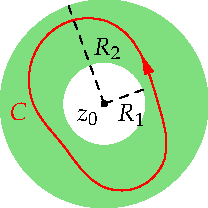
\includegraphics[scale=0.95]{laurent2}
\end{defn}


\begin{itemize}
  \item If you prefer, write $\sum\limits_{n=0}^\infty a_n(z-z_0)^n+\sum\limits_{n=1}^\infty \frac{b_n}{(z-z_0)^n}$ where $b_n=\frac 1{2\pi i}\oint_C(z-z_0)^{n-1}f(z)\,\dz$.\par
  \begin{minipage}[t]{0.73\linewidth}\vspace{0pt}
		\item The coefficients $a_n$ are independent of the choice of contour $C$.\smallbreak
		To see this, suppose $D$ is another simple closed curve encircling $z_0$, and choose a circle $E$ outside both $C$ and $D$. Since $\frac{f(z)}{(z-z_0)^{n+1}}$ is analytic on the annulus, two applications of Cauchy--Goursat yield
	  \[
	  	\oint_{\textcolor{red}{C}}\frac{f(z)}{(z-z_0)^{n+1}}\,\dz
	  	=\oint_{\textcolor{purple}{E}}\frac{f(z)}{(z-z_0)^{n+1}}\,\dz
	  	=\oint_{\textcolor{blue}{D}}\frac{f(z)}{(z-z_0)^{n+1}}\,\dz
	  \]
	\end{minipage}
	\hfill
	\begin{minipage}[t]{0.26\linewidth}\vspace{-5pt}
		\flushright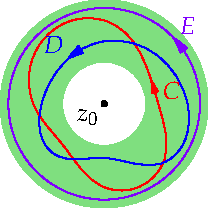
\includegraphics[scale=0.95]{laurent3}
	\end{minipage}\par
  
  \item If $f(z)$ is analytic on the \emph{disk} $\nm{z-z_0}<R_2$, then the Laurent series equals the Taylor series:
	\[
		\begin{cases}
			n\ge 0\implies a_n=\frac{f^{(n)}(z_0)}{n!} \quad &\text{(Cauchy's integral formula)}\\
			n<0\implies a_n=0 \quad &\text{(Cauchy--Goursat)}
		\end{cases}
	\]
\end{itemize}

\begin{example*}{\ref{ex:laurentmotiv}, cont.}{}
	$f(z)=\frac 1{z(2-z)}$ is certainly analytic on the \textcolor{blue}{annulus} $0<\nm z<2$.\par
	\begin{minipage}[t]{0.7\linewidth}\vspace{-4pt}
		By first writing $f(z)=\frac 12\left(\frac 1{z}+\frac 1{2-z}\right)$ using partial fractions, we compute the Laurent series for $f$ on the annulus using the \textcolor{Green}{unit circle} centered at the origin:
		\[
			a_n=\frac 1{2\pi i}\oint_C\frac{f(z)}{z^{n+1}}\,\dz =\frac 1{4\pi i}\oint_C \frac{1}{z^{n+2}}+\frac 1{(2-z)z^{n+1}}\,\dz
		\]
		The first integral evaluates to $\frac 12$ when $n=-1$ and to zero otherwise. The second  integral may be found using Cauchy's integral formula:
	\end{minipage}
	\hfill
	\begin{minipage}[t]{0.29\linewidth}\vspace{-4pt}
		\flushright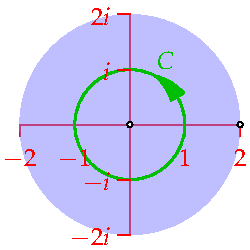
\includegraphics[scale=0.95]{laurent7}
	\end{minipage}\par
	\[
		\frac 1{4\pi i}\oint_C \frac 1{(2-z)z^{n+1}}\,\dz =
		\begin{cases}
			0&\text{if }n\le -1\\
			\displaystyle\frac 1{2(n!)}\diffat[{}^n]{z^n}{z=0}(2-z)^{-1} =\frac 1{2^{n+2}}&\text{if }n\ge 0
		\end{cases}
	\]
	We conclude that $a_n=\frac 1{2^{n+2}}$: the Laurent series of $f(z)$ is precisely the series computed previously!\smallbreak
	The Laurent series centered at $z_0=2$ can be computed similarly, both using the integral method and our original approach. 
\end{example*}

The example is typical. Computing a Laurent series directly from the definition is usually ugly given how many contour integrals must be evaluated! Thankfully, as we'll see shortly, all the standard facts regarding Taylor series translate to this new situation. In particular, if $f(z)=\sum a_n(z-z_0)^n$ equals a series with negative terms, then the series will turn out to be the Laurent series of $f(z)$. We'll deal with the theory shortly, but first a few more examples following from this observation to get used to the idea.



\begin{examples}{}{laurenteasyex}
	\exstart On the \textcolor{blue}{disk $\nm z<1$}, we have the Maclaurin series
	
	\begin{enumerate}\setcounter{enumi}{1}
	  \begin{minipage}[t]{0.73\linewidth}\vspace{-13pt}
		  \item[]%
		  \[
		  	\frac 1{z-i}=\frac 1{-i(1-\frac zi)}
		  	=i\sum_{n=0}^\infty(-iz)^n
		  	=i+z-iz^2-z^3+iz^4+\cdots
		  \]
			On the \textcolor{Green}{annulus $\nm z>1$}, we have the Laurent series
			\[
				\frac 1{z-i}=\frac z{(1-\frac iz)}
				=\sum_{n=0}^\infty i^nz^{-n-1}
				=\frac iz-\frac 1{z^2}-\frac i{z^3}+\frac 1{z^4}+\cdots
			\]
		
			\item On the \textcolor{orange}{$1<\nm z<2$}, we have the Laurent series
			\begin{align*}
				\frac 3{(2-z)(1+z)}
				&=\frac 1{2-z}+\frac 1{1+z}=\frac 1{2(1-\frac z2)}+\frac 1{z(1+\frac 1z)} \\
				&=\frac 12\sum_{n=0}^\infty\left(\frac z2\right)^n+\frac 1z\sum_{m=0}^\infty(-z)^{-m}\\
				&=\cdots +z^{-3}-z^{-2}+z^{-1}+\frac 12+\frac 14z+\frac 18z^2+\cdots
			\end{align*}
		\end{minipage}
		\hfill
		\begin{minipage}[t]{0.26\linewidth}\vspace{-20pt}
			\flushright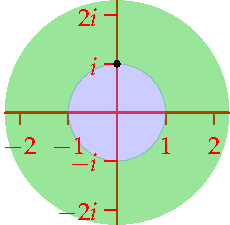
\includegraphics[scale=0.95]{laurent5}\bigbreak
			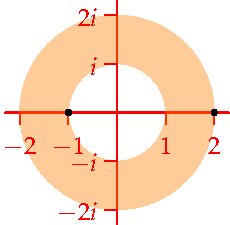
\includegraphics[scale=0.95]{laurent6}
		\end{minipage}\par	
		
	
	  \item Since $e^z=\sum \frac{z^n}{n!}$ is valid on the entire complex plane, we obtain the Laurent series expansion
	  \[
	  	e^{\frac 1z}=\sum_{n=0}^\infty\frac{z^{-n}}{n!}=1+\frac 1z+\frac 1{2z^2}+\frac 1{6z^3}+\cdots
	  \]
	  valid on the punctured plane $z\neq 0$.
	  
	  \item Again by substituting in a known Maclaurin series, we obtain another Laurent series valid on the punctured plane $z\neq 0$:
	  \[
	  	\frac 1{z^7}\sin z^2
	  	=\sum_{n=0}^\infty\frac{(-1)^n}{(2n+1)!}z^{4n-5} 
	  	=z^{-5}-\frac 16z^{-1}+\frac 1{120}z^3-\frac 1{5040}z^7+\cdots
	  \]
	  
	  \item Multiplying term-by-term, and since we need \emph{both} Maclaurin series to be valid, we obtain (the first few terms of) a Laurent series valid on the punctured disk $0<\nm z<1$:
	  \begin{align*}
		  \frac 1{z(z-1)(z-2i)}&=\frac 1z\left(\sum_{n=0}^\infty (-1)^nz^n\right)\left(\sum_{m=0}^\infty\left(\frac i2\right)^mz^m\right)\\
		  &=\frac 1z\left(1-z+z^2-z^3+\cdots\right)\left(1+\frac i2z-\frac 14z^2-\frac i8z^3+\cdots\right)\\
		  &=\frac 1z+\left(-1+\frac i2\right)+\left(\frac 34-\frac i2\right)z+\left(-\frac 34+\frac{3i}8\right)z^2+\cdots
	  \end{align*}
	\end{enumerate}
\end{examples}

\goodbreak


%\boldsubsubsection{Theory time!}

We now state and prove the main properties of Laurent series. These are very similar to the corresponding statements \& arguments for Taylor series; the additional challenge mostly comes from keeping track of two series at once.

\begin{thm}{Laurent's Theorem}{}
	An analytic function on an open annulus equals its Laurent series.
\end{thm}

\begin{proof}
	It is enough to prove when the annulus is centered at $z_0=0$. Let $w$ in the annulus be given.\par
	\begin{minipage}[t]{0.73\linewidth}\vspace{-3pt}
		Since the annulus is open, we may choose three non-overlapping circles $\alpha,\beta,\gamma$ with radii $R_\alpha,R_\beta,R_\gamma$ as in the picture:
		\begin{itemize}
		  \item $\gamma$ a \textcolor{Green}{small circle} centered at $w$ inside the annulus;
		  \item $\alpha,\beta$ centered at 0, \textcolor{red}{$\alpha$ inside} and \textcolor{orange}{$\beta$ outside} $w$ (thus $R_\alpha<\nm w<R_\beta$). 
		\end{itemize}
		Since $\frac{f(z)}{z-w}$ is analytic on the region inside $\beta$ with interior boundaries $\alpha$ and $\gamma$, Cauchy--Goursat and the integral formula tell us that
	\end{minipage}
	\hfill
	\begin{minipage}[t]{0.25\linewidth}\vspace{-4pt}
		\flushright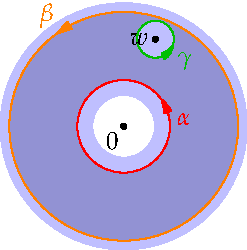
\includegraphics[scale=0.95]{laurent4}
	\end{minipage}\par
	\[
		\left(\oint_\beta-\oint_\alpha-\oint_\gamma\right)\frac{f(z)}{z-w}\,\dz=0\implies f(w)=\frac 1{2\pi i}\oint_\gamma\frac{f(z)}{z-w}\,\dz =\frac 1{2\pi i}\left(\oint_\beta-\oint_\alpha\right)\frac{f(z)}{z-w}\,\dz
		\tag{$\ast$}
	\]
	As in the proof of Taylor's theorem, we expand $\frac 1{z-w}$, this time in two ways:
	\[
		\frac 1{z-w}
		=\frac 1z\sum_{k=0}^{n-1}\left(\frac wz\right)^k +\frac 1{z-w}\left(\frac wz\right)^n 
		=-\frac 1w\sum_{k=1}^{n}\left(\frac zw\right)^{k-1} +\frac 1{z-w}\left(\frac zw\right)^n
	\]
	These expansions allow us to attack the two integrals in ($\ast$):
	\begin{gather*}
		\frac 1{2\pi i}\oint_\beta\frac{f(z)}{z-w}\,\dz
		=\sum_{k=0}^{n-1}\underbrace{\frac{w^k}{2\pi i}\oint_\beta \frac{f(z)}{z^{k+1}}\,\dz}_{a_kw^k} +\frac{w^n}{2\pi i}\oint_\beta \frac{f(z)}{z^n(z-w)}\,\dz\\
		\frac{-1}{2\pi i}\oint_\alpha\frac{f(z)}{z-w}\,\dz =\sum_{k=1}^{n}\underbrace{\frac 1{2\pi iw^k}\oint_\alpha z^{k-1}f(z)\,\dz}_{a_{-k}w^{-k}} -\frac 1{2\pi i w^n}\oint_\alpha \frac{z^nf(z)}{z-w}\,\dz
	\end{gather*}
	We finish by summing and estimating, using the facts that $z\in\alpha\cup\beta\Longrightarrow\nm{z-w}>R_\gamma$, and that $f(z)$ is bounded (by some $M>0$) on the closed bounded annulus between $\alpha,\beta$:
	\begin{align*}
		\nm{f(w)-\sum_{k=-n}^{n-1}a_kw^k}
		&=\nm{\frac{w^n}{2\pi i}\oint_\beta \frac{f(z)}{z^n(z-w)}\,\dz -\frac 1{2\pi iw^n}\oint_\alpha \frac{z^nf(z)}{z-w}\,\dz}\\
		&\overset{\triangle}{\le} \frac{\nm w^n}{2\pi}\nm{\oint_\beta \frac{f(z)}{z^n(z-w)}\,\dz} +\frac 1{2\pi\nm w^n}\nm{\oint_\alpha \frac{z^nf(z)}{z-w}\,\dz}\\
		&\le \frac{\nm w^n}{2\pi}\cdot\frac{M}{R_\beta^nR_\gamma}\cdot 2\pi R_\beta +\frac 1{2\pi\nm w^n}\cdot \frac{R_\alpha^nM}{R_\gamma}\cdot 2\pi R_\alpha
			\tag{Theorem \ref{thm:intbound}}\\
		&=\frac M{R_\gamma}\left[R_\beta\left(\frac{\nm w}{R_\beta}\right)^n+R_\alpha\left(\frac{R_\alpha}{\nm w}\right)^n\right] \xrightarrow[n\to\infty]{} 0
		\tag*{\qedhere}
	\end{align*}
\end{proof}

\goodbreak


% \begin{defn}{}{}
% 	Given a series $\smash[b]{f(z)=\sum\limits_{n=-\infty}^\infty a_n(z-z_0)^n}$, define
% 	\[
% 		R_1=\inf\bigl\{\nm{z-z_0}:f(z)\text{ converges}\bigr\},\qquad 
% 		R_2=\sup\bigl\{\nm{z-z_0}:f(z)\text{ converges}\bigr\}
% 	\]
% 	The region $R_1<\nm{z-z_0}<R_2$ is called the (open) \emph{annulus of convergence.}
% \end{defn}

Our final corollary summarizes the remaining core properties of Laurent series.


\begin{cor}{}{laurenttidy}
	Let $f(z)=\sum a_n(z-z_0)^n$ be a series. Then:
	\begin{enumerate}
% 	  \item On its open annulus of convergence, $f(z)$ converges absolutely to a continuous function. As with power series, convergence on the boundary circles must be checked separately.
% 	  \item The convergence is uniform on any closed sub-annulus.
  	\item\label{cor:laurtidy3} (Term-by-term Integration)\quad If $g(z)$ is continuous on a contour $C$ lying inside the annulus, then
  	\[
  		\int_C g(z)f(z)\,\dz=\sum_{n=-\infty}^\infty a_n\int_Cg(z)(z-z_0)^n\,\dz
  	\]
  	In particular, $f(z)$ may be integrated term-by-term along $C$.
 
 		\item\label{cor:laurtidy4} (Analyticity/Derivatives)\quad $f(z)$ is analytic on the annulus and $f'(z)=\sum\limits_{n=-\infty}^\infty a_nn(z-z_0)^{n-1}$
  	
  	\item\label{cor:laurtidy5} (Uniqueness)\quad $\sum a_n(z-z_0)^n$ is the Laurent series of $f(z)$ \ (as in Definition \ref{defn:laurent}).
	\end{enumerate}
\end{cor}

 The remainder are the analogues of Theorems \ref{thm:inttermbyterm} and Corollary \ref{cor:contintdiff}: some details are in Exercise \ref{exs:laurenttidy}.


\begin{examples}{}{}
	The corollary formally justifies Examples \ref{ex:laurenteasyex}. Here are two extensions.
	\begin{enumerate}
	  \item In accordance with part \ref*{cor:laurtidy4} of the corollary,
		\begin{align*}
			\frac 1{z^2}e^{1/z}
			&=-\diff ze^{1/z}=\diff z\sum_{n=0}^\infty\frac{z^{-n}}{n!} 
			=\sum_{n=1}^\infty\frac{z^{-1-n}}{(n-1)!} 
			=\frac 1{z^2}\sum_{n=1}^\infty\frac{z^{-(n-1)}}{(n-1)!} 
			=\frac 1{z^2}\sum_{n=0}^\infty\frac{z^{-n}}{n!}\\
			&=\frac 1{z^2}+\frac 1{z^3}+\frac 1{2z^4}+\frac 1{6z^5}+\frac 1{24z^6}+\cdots
		\end{align*}
		We need not have differentiated: by part \ref*{cor:laurtidy5} we could instead simply multiply the known series for $e^{1/z}$ term-by-term to obtain the result!
		\item We use part \ref*{cor:laurtidy3} to compute the integral around a contour $C$ encircling the origin:
		\[
			\oint_C\frac 1{z^7}\sin z^2\,\dz =\sum_{n=0}^\infty\frac{(-1)^n}{(2n+1)!}\oint_Cz^{4n-5}\,\dz =\oint_C\frac{(-1)^1}{(2+1)!}z^{4-5} =-\frac 13\pi i
		\]
		since all but one of the integrals evaluates to zero.
	\end{enumerate}
\end{examples}

\goodbreak

\begin{exercises}
	\exstart (Example \ref{ex:laurentmotiv}, cont.)\lstsp $f(z)=\frac 1{z(2-z)}$ is analytic everywhere except $z=0$ and $z=2$.\vspace{-5pt}

	\begin{enumerate}\setcounter{enumi}{1}
	  \item[]\begin{enumerate}
	    \item Use Definition \ref{defn:laurent} to directly compute the Laurent series of $f(z)$ on the punctured disk $0<\nm{z-2}<2$ using the circle radius 1 centered at $z_0=2$.
	    \item Use the Taylor series of $\frac 1z$ centered at $z_0=2$ to more rapidly find the Laurent series in (a).
	  \end{enumerate}
	  
	  
	  \item Find a Laurent series representation for each function. Also find $\oint_Cf(z)\,\dz$ where $C$ is a simple closed curve in the given domain encircling the origin.
	  \begin{enumerate}
	    \item $f(z)=\frac 3{z^2}e^{2z}$ whenever $\nm z>0$
	   
	    \item $f(z)=\cos\frac iz$ whenever $\nm z>0$
	    
	    \item $f(z)=\frac 1{1+z^3}$ when $1<\nm z$\quad (\emph{Hint: let $w=z^{-1}$})
	  \end{enumerate}
	  
	  \goodbreak
	  
	  \item On each domain, find a Laurent series centered at $z_0=0$ for the function
	  \[
	  	f(z)=\frac{1}{z(z-2i)}=\frac i2\left(\frac 1z-\frac 1{z-2i}\right)
	  \]
	  \begin{enumerate}
	    \item $D_1=\{z:0<\nm z<2\}$
	    \qquad\qquad
	    (b) \ $D_2=\{z:\nm z>2\}$ \ (\emph{again let $w=z^{-1}$})
		\end{enumerate}
		
		
		\item Repeat the previous question for
	  \[
	  	f(z)=\frac{1-2i}{(z-1)(z-2i)}=\frac 1{z-1}-\frac 1{z-2i}
	  \]
	  Also find $\oint_Cf(z)\,\dz$ where $C$ is a simple closed curve in the given domain encircling the origin.
	  \begin{enumerate}
	    \item $D_1=\{z:0<\nm z<1\}$
	    \qquad\quad% (\emph{this is a Taylor series})
	    (b) \ $D_2=\{z:1<\nm{z}<2\}$
			\qquad\quad
			(c) \ $D_3=\{z:\nm z>2\}$
		\end{enumerate}
	
	
		\item Show that when $0<\nm{z-1}<2$,  we have
		\[
			\frac z{(z-1)(z-3)}=-\frac 1{2(z-1)}-3\sum_{n=0}^\infty\frac{(z-1)^n}{2^{n+2}}
		\]
		
		
		\item Let $a$ be complex number. Show that
		\[
			\frac a{z-a}=\sum_{n=1}^\infty\frac{a^n}{z^n}
			\quad\text{whenever }
			\nm a<\nm z
		\]
		
		
	  \item\label{exs:laurenttidy} Suppose $f(z)=\sum a_n(z-z_0)^n$ is a series as in Corollary \ref{cor:laurenttidy}.
	  \begin{enumerate}
	    \item Suppose part \ref*{cor:laurtidy3} has been proved. Explain why the function $f(z)-a_{-1}(z-z_0)^{-1}$ is analytic on the annulus. Hence conclude that $f(z)$ is analytic on the annulus.\par
	    (\emph{This is different to Corollary \ref{cor:contintdiff} since $a_{-1}(z-z_0)^{-1}$ has no anti-derivative on the annulus!})
	    \item In order to mimic the proof of Corollary \ref{cor:contintdiff} to show that $f(z)$ is differentiable term-by-term, what properties must the curve $C$ have?
	    \item Prove part \ref*{cor:laurtidy5}.\par
	    (\emph{Hint: Recall Exercise \ref*{sec:unifconv}.\ref{ex:uniquetaylor} - the same hint works!}).
		\end{enumerate}
	\end{enumerate}
\end{exercises}

